\subsection{Optimal Recognition Position} \label{ORP}
The destination of each saccade when reading, or the fixation point, depends on the content of the sentence; sometimes, the eye also skip words by saccading past them. 80\% of the fixation points are on content words (nouns, verbs and adjectives) and the remaining 20\% are on articles, pronouns, and conjunctions \cite{eysenck_cognitive_2010}. The fixation point inside the words themselves, the \textit{optimal recognition position} (ORP), has an impact on how fast a reader can name the word they are looking at. Research has shown that the ORP is near the middle or slightly left of the middle \cite{oregan_optimal_1992, nazir_letter_1998, oregan_convenient_1984}. The added recognition time as the fixation point deviates from the ORP is a U-shaped curve (see Figure \ref{fig:ucurve}), with around 20 ms added for each letter of deviation.

\begin{figure}[htbp]
\centering
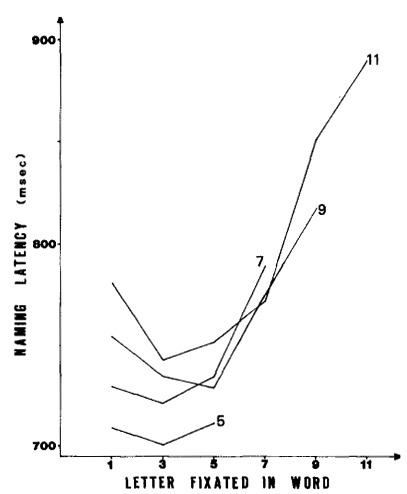
\includegraphics[width=0.4\textwidth]{Pics/ucurve}
\caption{The time it took participants to name a word depending on their fixation point. This graph shows results for words of length 5, 7, 9, and 11. For example, when reading a five-letter word, the ORP is 3. \protect\cite{oregan_convenient_1984}}
\label{fig:ucurve}
\end{figure}

Removing the spacing between words decreases the reading speed with around 30\% \cite{eyeMovement}. Fixation does not fall on the ORP, but tends to the beginning of words. Splitting long words, like long Danish or German compound words, into individual words increases the reading speed, even though it is grammatically incorrect. Likewise, inserting spaces in Thai (where there's normally no spaces), also increases reading speed 	\cite{eyeMovement}.